\chapter{Materials and methods}
% \thispagestyle{fancy}

Based on the former literature review, the technical route of this degree project was designed as the flow chart showed in Figure \ref{flow-chart}. In the eQTL analysis, the genotypes and gene expression of the tumor tissue were used. The somatic mutations were also identified using DNA sequencing data from both tumor tissues and matched normal tissues. The overlapped genes between somatically mutated genes and the eGenes identified through eQTL analysis were defined as potential driver eGenes that hold higher potential for triggering cancer development. After excluding the overlapped eGenes between the GTEx portal and this study, the eGenes specific to this Japanese cancer cohort can be identified.


\begin{figure}[h]
\centering
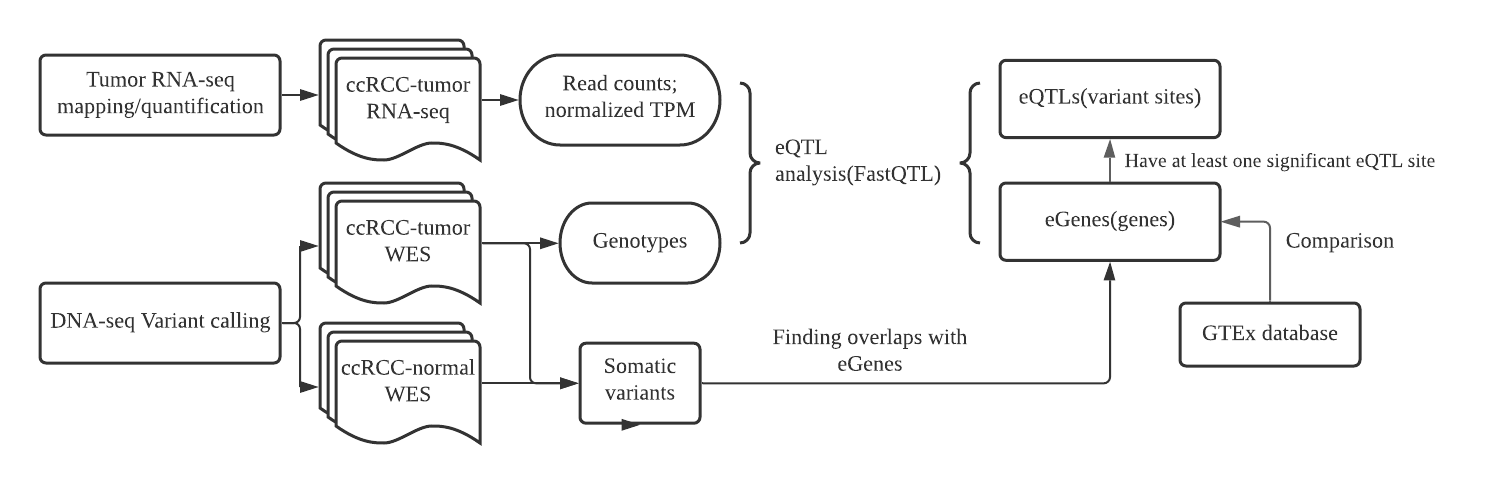
\includegraphics[width=1.0\textwidth]{figures/eQTL-analysis (3).png}
\caption{Study flow in this degree project}
\label{flow-chart}
\end{figure}

This project used both DNA-sequencing and RNA-sequencing data from 100 ccRCC patients from Asia(Japan), which originated from an integrated research from Japan\cite{sato_integrated_2013}. All the sequence data were in bam format and downloaded from the European genome-phenome archive, coded with EGAD00001000597.The DNA-sequencing data contains tumor data from ccRCC tumor specimens and matched normal data from either normal kidney tissue(97 patients) or peripheral blood(3 patients). The DNA-sequencing used SureSelect targeted sequencing which performed by Illumina HiSeq 2000 platform with 100-bp paired-end reads. Based on the original dataset description, the mean depths of coverage of the entire targeted regions were 129×. The RNA-sequencing was performed on the same platform for 100 ccRCC cases. The data analysis was handled mostly by Uppmax platform and some by Docker images provided by GTEx.\\

The cohort consists of 23 females and 77 males and the ages are widely distributed between 35 to 91. The patient's condition was recorded in the metadata, majorly includes the stage at diagnosis, Fuhrman grade, metastases, and outcome(dead/alive). Some metadata were used in generating covariates in eQTL analysis.

See the table \ref{tab:sample-table} for a summary of used data set.

\begin{table}[!ht]
\centering
\caption{A summary of dataset used in this project}
~\\
\label{tab:sample-table}
\begin{tabular}{lll}
\toprule
\textbf{SAMPLE}		  &\textbf{Sequencing method}	& \textbf{Amount}                                                                                                                                                  \\ \toprule
ccRCC Tumor                &Whole exome sequencing  & 100 \\
\midrule
ccRCC Normal 	& Whole exome sequencing & 100 \\
\midrule
ccRCC Tumor         & RNA-sequencing        & 100\\
\bottomrule
\end{tabular}
\end{table}



\section{RNA-sequencing and quantification}

The processing of RNA-sequencing data followed the GTEx portal with some parameter adjustment based on the ccRCC dataset.

The index for STAR(v2.5.3a)\cite{dobin_star_2013} was built with matched sequencing read length 100bp. The genome file GRCh38/hg38 and the annotation file GENCODE v26 was used.The downloaded BAM files were transformed to paired fastq files using Picard(http://broadinstitute.github.io/picard/)function SamToFastq. The FASTQ format paired-files were aligned to GRCh38/hg38 reference genome using STAR(v2.5.3a) \cite{dobin_star_2013}. STAR were set to two-pass mode and the results have been sorted by coordinate using samtools(http://www.htslib.org/). The duplicates were removed using Picard function MarkDuplicates.The gene-level quantification was generated use RNA-SeQC2.3.6(https://github.com/getzlab/rnaseqc). During the process, the read-level filters were applied automatically by RNA-SeQC to ensure well quantification. The RNA-seq data were performed by unstrand-specific sequencing. The related collapsed-gene model that combined all isoforms of a gene into a single transcript was used as an input file for RNA-SeQC. The file is available in GTEx resources(https://console.cloud.google.com/storage/browser/gtex-resources/GENCODE). The outputs for 100 samples were combined into one union file and prepared for eQTL analysis.


\section{DNA-sequencing processing and mutations calling}

The processing pipeline of DNA-sequencing data was based on The Genome Analysis Toolkit (GATK) 4.1.1.0\cite{mckenna_genome_2010}'s best practice. Several details have been adjusted using GTEx published literature\cite{noauthor_gtex_2020}'s supplementary materials as a guide.


\subsection{Pre-processing for variant discovery} 
In this step, the raw bam files were all converted into FASTQ files and re-mapped to hg38 using BWA-MEM. The read group information was added using Picard. In order to improve the quality of variant calling, local realignment (using GATK IndelRealigner) was applied first. The GATK's duplicates removal and base quality score recalibration were then applied to all the 200 BAM files.

\subsection{Variants calling on tumor samples} 
GATK HaplotypeCaller was applied to call all the appeared variants (SNVs, Indels) from each tumor sample. The variants for 100 samples were joint-called using GATK GenomicsDBImport and GenotypeGVCFs. The variants were restricted to chromosomes 1-22 and chromosome X. 

\subsection{Variants quality control}
The variants were filtered based on multiple steps listed below. 

1)Variant (Quality Score) Recalibration (VQSR) with allele-specific mode. This mode took consideration of multi-allelic sites. Before VQSR, a hard filter for Excess heterozygosity(ExcessHet) > 54.69 was applied considering a relativey large cohort size(100). The VQSR step calculated a model using machine learning and applied a threshold of 99.8\% (for SNPs) and 99.95\%(for Indels) to filter the variants.

2)Applied hard-filtering at site-level. Firstly, the sites with QUAL <30 or QualByDepth(QD) <2.0 threshold were filtered out. As an explaination, QUAL value is the Phred-scaled quality score and QD is the QUAL score normalized by Depth. Then the sites with low Inbreed Coefficient < -0.3 were filtered out. An Inbreed Coefficient value of 0 means that the site is in Hardy-Weinberg equilibrium. But negative value indicating that the sites were with bad mapping. The value of -0.3 was chosen to align with GTEx.

3) For filtration at the genotype level, the sum VCF file of 100 samples was processed through the GATK genotype refinement pipeline to re-calculate the GQ value per sample at per variant site. The variants from the 1000 Genomes project were used as a supporting file. The genotypes with re-calculated GQ <20 or the minimum read depth (DP) <3 were filtered using GATK VariantFiltration. After this filtration, the total variant sites were not changed but the unqualified genotypes were all set to missing(shown as "./.")

4) In order to continue downstream quality control, the multi-allelic sites were split into biallelic sites using Hail 0.2 (https://hail.is/).

5) After splitting, the monomorphic SNPs that have no called alternative alleles (AC==0) were removed using bcftools(https://samtools.github.io/bcftools/)filter. AC is the allele count in genotypes for the “ALT” allele(s).

6) The missingness of genotypes at each site was set to the maximum tolerance of 0.25, which means only the variant sites that called in more than 75\%  of individuals were kept. This step used bcftools for filtration and it ensured convincing genotype results to be used in eQTL analysis. The threshold is less strict than the threshold that GTEx used (0.15), but still filtered out most of the variants.

7) The threshold of minor allele frequencies (MAF) was set to <= 0.01 using bcftools , which means a variant site was excluded if its minor allele is found in equal or less than 1\% genotypes. 

See Table \ref{tab:Mutation_filter_step} for a detailed number of variants in different filtering process.
\begin{table}[!ht]
\centering
\caption{Variants QC filtering from Haplotypecaller}
~\\
\label{tab:Mutation_filter_step}
\begin{tabular}{lll}
\toprule
\textbf{Filtering / processing criterion}		  & \textbf{Total sites}   &\textbf{Percentage}                                                                                                                                       \\ \toprule
Initial variants                   & 7088610	&100.00\%	\\
\midrule
VQSR and ExcessHet not PASS & 6813720 	&96.12\%	\\
\midrule
QD <2.0 or QUAL <30 & 6804941	&96.00\%	\\
\midrule
InbreedingCoeff < -0.3  & 6802902	&95.97\%	\\
\midrule
Hail splitting Multi-allelic sites 	& 6927794 	&\\
\midrule
Monomorphic sites with AC =0 & 6356484	&89.67\% \\
\midrule
Missingness > 25\% & 459062	&6.48\% \\
\midrule
MAF <=1\% & 284774	& 4.02\% \\ 
\bottomrule
\end{tabular}
\end{table}


\subsection{Somatic mutations identification using tumor samples and matched normal}
The GATK Mutect2 was applied to prepared tumor BAM files and matched normal BAM files to identify somatic variants. While using the 'Tumor with matched normal' model, a panel of normal(PON) file provided by GATK was also used to filter the germline variants. FilterMutectCalls was used to filter the somatic mutations which considered read orientation bias and cross-contamination.\\

\subsection{Mutations annotation}

The mutation files were first annotated using GATK VariantAnnotator using dbsnp138 databases. Then the SnpEff\cite{cingolani_program_2012}(http://pcingola.github.io/SnpEff/) was used for a detailed functional annotation.

\section{Japanese cohort eQTL analysis}

The mapping strategy in FastQTL is based on linear regression. For a simple linear regression, the gene expression is the response variable while only genotypes of each sample are included as explanatory variables that affect the value of gene expression. The formula is as follows: $$ Y_i=\beta_0+\beta x_i+\epsilon_i $$

The multiple linear regression uses several explanatory variables to predict the outcome of response variable, which make it possible to consider other possible factors such as sex, gender and other types of independent variables. Those factors could input as covariates when perform linear regression using FastQTL.The formula is as follows:$$ Y_i=\beta_0+\beta_1 x_{i1}+\beta_2 x_{i2}+ ... + \beta_p x_{ip}+\epsilon_i $$  

In the two formulas,  $Y_i $ represents the gene expression, and $x_i$ represents all the factors that might regulate the gene expression, including genotypes and covariates of each sample.

When testing the associations between genes and variants, for a single gene, there are series of variants inside the cis window (Within 1 Megabase for both upstream and downstream from the transcription start site). Millions of association tests were used to scan all the phenotype-variant pairs, which is called a 'norminal pass' in FastQTL. Due to the large amounts of tests performed, a multiple testing correction is needed to assess the significance of candidate variants. The correction is achieved by analyzing a range of permuted datasets per phenotype, which is called a 'permutation pass' in FastQTL.

To perform the eQTL analysis using software FastQTL\cite{ongen_fast_2016}, several steps were used for preparation. The environment was prepared based on a Docker image provided by GTEx.The gene-level expression data for 100 patients were normalized based on the same principle with GTEx.The sample id appeared in DNA-sequencing and RNA-sequencing for the same individual was mapped in a list as a reference for eQTL mapping. A cis-mapping windows range was set to within 1Mb between variants and genes.The variant IDs were set using variants information(chromosome, position,REF,ALT). An adaptive permutation pass between 100 to 1000 times was used to get the adjusted p-value for each site.The missing genotypes were imputed when FastQTL starts to read the genotype data file. Extra gene and variant information were added to the final eQTL results.

\subsection{Covariates generation}
Covariates that combined in different aspects were used in FastQTL. In order to estimate hidden determinants of gene expression, the probabilistic estimation of expression residuals (PEER)\cite{stegle_using_2012}were used. The number of PEER factors(15) was set based on the sample size(100). Usually, the top 5 PC components from PCA analysis across all the filtered genotypes were used for population stratification. All the samples from the Japanese cohort theoretically have the same genetic ancestry. Nevertheless, the first 5 PCs calculated using PLINKv1.9\cite{purcell_plink_2007} were still included in the covariates file. The sex and age factor(below 50 years old or above) were considered as part of covariates. Finally, the patient's stage of diagnosis which recorded by the metadata was included as covariates in the following rules:  the information of tumor size(T) has been encoded as numbers from 1 to 4; whether cancer has spread into nodes(N) or not has been encoded as numbers 0,1 or 2(represents an extent of spread);  whether cancer has spread to distant tissues, named metastasis situation (M)  and has been encoded as 0 or 1. The FastQTL was run by both nominal-pass and permutation-pass. A minor allele sample count threshold of at least 10 samples was set when running FastQTL.

\subsection{Gene set enrichment analysis}

The gene set enrichment analysis for a list of significant eGenes was achieved by the web-based tool Enrichr\cite{kuleshov_enrichr_2016} with default setting. 

\section{GTEx kidney tissue eQTLs data acquision}

The eQTLs analysis results (V8 release) for all the tissues are available at GTEx portal(https://www.gtexportal.org/home/datasets).The kidney tissue-specific eQTL data were downloaded and extracted for downstream comparison. In order to obtain a list of significant eGenes, only eGenes with a q value lower than 0.05 were collected.

\section{Boxplot of eQTLs and eGenes}

The boxplot that described how the genotype affects corresponding gene expression for Japanese cohort results was drawn using an R script provided in appendices\ref{sec:Appendices}. The genotypes have been transformed using following rules: The genotypes with 0/0 were changed to value 0; the genotypes with 0/1 were changed to value 1; the genotypes with 1/1 were changed  to value 2. The missing genotypes with ./. were set to value 0. 

